%! suppress = TooLargeSection
% -*- TeX:SI -*-
% slovene sub-mode for spell check
%%%%%%%%%%%%%%%%%%%%%%%%%%%%%%%%%%%%%%%%%%%%%%%%%%%%%%%%%%%%%%%%%%%%%%%%%%%%%%%%%%%%%%%%%%%%%%%%%%%%%%%%%%%%%%%%%%%%%%%%
% LaTeX predloga za zaključna dela
% Univerza v Ljubljani, Fakulteta za elektrotehniko
% Zbral in uredil: Roman Kamnik, junij 2013
% Dopolnil: Sebastjan Šlajpah (2013), Sašo Tomažič (2013), Peter Miklavčič (2019)
%%%%%%%%%%%%%%%%%%%%%%%%%%%%%%%%%%%%%%%%%%%%%%%%%%%%%%%%%%%%%%%%%%%%%%%%%%%%%%%%%%%%%%%%%%%%%%%%%%%%%%%%%%%%%%%%%%%%%%%%
\documentclass[a4paper,twoside,openright,12pt,slovene]{book}
\usepackage[pdftex]{UNI-LJ-FE-Diploma} % stil zaključnega dela UL FE
\usepackage{lmodern} % Alternativna pisava, izgleda bolje ko vklopiš T1 fontenc
\usepackage[utf8]{inputenc} % predloga uporablja standardno kodiranje Unicode UTF-8, ki podpira šumnike
\usepackage[greek,english,slovene]{babel} % seznam uporabljenih jezikov (zadnji na seznamu je primarni)
\usepackage[T1]{fontenc} % Podpora pisavam z več simboli, omogoča direktno kopiranje šumnikov

% PDF/A %%%%%%%%%%%%%%%%%%%%%%%%%%%%%%%%%%%%%%%%%%%%%%%%%%%%%%%%%%%%%%%%%%%%%%%%%%%%%%%%%%%%%%%%%%%%%%%%%%%%%%%%%%%%%%%%
% Več o PDF/A v LaTeX-u: https://www.mathstat.dal.ca/~selinger/pdfa/
\usepackage{filecontents}
\begin{filecontents*}{\jobname.xmpdata}
    \Title{Izdelava in ovrednotenje regenerativnega polnilnika in preizkuševalnika Li-ion baterij} % Mora biti enak kot je v prijavi teme!
    \Author{Sašo Domadenik} % Mora biti enak kot na naslovnici!
\end{filecontents*}
\usepackage[a-1b]{pdfx}
%%%%%%%%%%%%%%%%%%%%%%%%%%%%%%%%%%%%%%%%%%%%%%%%%%%%%%%%%%%%%%%%%%%%%%%%%%%%%%%%%%%%%%%%%%%%%%%%%%%%%%%%%%%%%%%%%%%%%%%%

% LaTeX PAKETI %%%%%%%%%%%%%%%%%%%%%%%%%%%%%%%%%%%%%%%%%%%%%%%%%%%%%%%%%%%%%%%%%%%%%%%%%%%%%%%%%%%%%%%%%%%%%%%%%%%%%%%%%
% Kompakten pregled LaTeX ukazov je dostopen na https://en.wikibooks.org/wiki/Category:Book:LaTeX
% Navodila posameznih uporabljenih paketov so dostopna na https://www.ctan.org

% Dodatni simboli
\usepackage{textcomp}                               % dodatni simboli (kot npr. €)
\usepackage{gensymb}                                % dodatni simboli \de­gree, \cel­sius, \pert­hou­sand, \mi­cro, \ohm
\newcommand{\uppi}{\textrm{\greektext p\latintext}} % velika grška črka P z \uppi, alternativa simbolu \Pi

% Osnovno oblikovanje
\hypersetup{unicode,hidelinks,breaklinks,hyperindex} % dodatne možnosti hiperpovezav
\usepackage[normalem]{ulem}                          % podčrtavanje in prečrtavanje teksta
\usepackage{float}                                   % dodatne možnosti oblikovanja objektov
\usepackage{enumitem}                                % dodatne možnosti oblikovanja seznamov

% Dodatno oblikovanje
%\zamaknirobsodihstrani{0mm} % dodatna prilagoditev levega roba sodih strani za dvostranski tisk
%\usepackage{dcolumn}        % poravnava po decimalnih mestih v tabelah
%\usepackage{longtable}      % večstranske tabele
%\usepackage{caption}        % dodatne možnosti označevanja objektov
%\usepackage{rotating}       % vretenje objektov, strani, ipd.4
\usepackage{multirow}

% Matematična orodja
\usepackage{mathtools} % http://mirrors.ctan.org/macros/LaTeX/contrib/mathtools/mathtools.pdf
\usepackage{bm}        % ukaz za odebeljeni tisk \bm v matematičnih okoljih
%\usepackage{cancel}   % ukaz za prečrtavanje \cancel v matematičnih okoljih

% Grafična orodja
%\usepackage{graphicx}                % vključevanje bitnih slik z ukazom \includegraphics // Že vključen v .sty
\usepackage{grffile}                  % podpora presledkom pri ukazu \includegraphics
\usepackage{tikz}                    % paket TikZ za risanje (npr. blokovnih shem, diagramov poteka, itd.)
%\usetikzlibrary{calc,shapes,arrows}  % dodatne možnosti paketa TikZ
%\usepackage{tikzscale}               % skaliranje risb
%\usepackage[smartlabels]{circuitikz} % risanje shem vezij
\usepackage{pgfplots}                % paket PGFPlots za risanje grafov, tudi iz CSV in podobnih datotek
\pgfplotsset{width=12cm,compat=1.18}
%\usepgfplotslibrary{polar,external}  % dodatne možnosti paketa PGFPlots
%\usepackage{tikz-3dplot}             % 3D risanje
% Primeri: http://texample.net , http://pgfplots.net/tikz/examples , http://pgfplots.sourceforge.net/gallery.html

% Vključevanje datotek
\usepackage{pdfpages}  % vključevanje PDF datotek z ukazom \includegraphics
%\usepackage{epstopdf} % vključevanje EPS datotek z ukazom \includegraphics // Že vključen v .sty
\usepackage{listings}  % orodja za izpisovanje programske kode
\lstset{               % nastavitve orodja za izpisovanje programske kode
    basicstyle=\ttfamily\footnotesize,
    breaklines=true,
    numbers=left,
    numberstyle=\scriptsize,
    keywordstyle=\color{blue},
    commentstyle=\color{unilj},
    stringstyle=\color{olive},
}

% Povezave znotraj dokumenta
\usepackage{hyperref}
\usepackage[all]{hypcap}

%%%%%%%%%%%%%%%%%%%%%%%%%%%%%%%%%%%%%%%%%%%%%%%%%%%%%%%%%%%%%%%%%%%%%%%%%%%%%%%%%%%%%%%%%%%%%%%%%%%%%%%%%%%%%%%%%%%%%%%%

% TEMNI NAČIN %%%%%%%%%%%%%%%%%%%%%%%%%%%%%%%%%%%%%%%%%%%%%%%%%%%%%%%%%%%%%%%%%%%%%%%%%%%%%%%%%%%%%%%%%%%%%%%%%%%%%%%%%%
% Za elemente, ki se morajo v temnem načinu spremeniti se uporabi:
% \ifdark
%     Temni način
% \else
%     Svetli način
% \fi

\newif\ifdark   % Definicija stikala za temni način
%\darktrue       % Vklop temnega načina

% Sprememba osnovnih barv dokumenta
\usepackage{xcolor}
\usepackage{color}
\ifdark
    \definecolor{bgcolor}{rgb}{0.17,0.17,0.17}
    \pagecolor{bgcolor}
    \color{white}
    \newcommand{\srcpath}{res_dark}
\else
    \definecolor{bgcolor}{rgb}{1,1,1}
    \newcommand{\srcpath}{res}
\fi

\definecolor{plotcolor1}{HTML}{F44336}
\definecolor{plotcolor2}{HTML}{2196F3}
%%%%%%%%%%%%%%%%%%%%%%%%%%%%%%%%%%%%%%%%%%%%%%%%%%%%%%%%%%%%%%%%%%%%%%%%%%%%%%%%%%%%%%%%%%%%%%%%%%%%%%%%%%%%%%%%%%%%%%%%

% DEKLARACIJE %%%%%%%%%%%%%%%%%%%%%%%%%%%%%%%%%%%%%%%%%%%%%%%%%%%%%%%%%%%%%%%%%%%%%%%%%%%%%%%%%%%%%%%%%%%%%%%%%%%%%%%%%%
\naslov{Izdelava in ovrednotenje regenerativnega polnilnika in preizkuševalnika Li-ion baterij} % Mora biti enak kot je v prijavi teme!
\avtor{Sašo Domadenik} % Mora se ujemati s \Title pri metapodatkih PDF/A!
\mentor{prof. ddr. Iztok Humar}
%\somentor{Naziv, ime in priimek somentorja}
\date{Ljubljana, \the\year}
\univerza{Univerza v Ljubljani}
\definecolor{unilj}{cmyk}{0.00, 0.94, 0.94, 0.06} % barva Univerze v Ljubljani

% Potrebno je paziti, da je izbrana prava kombinacija tipa dela in sodelujočih fakultet glede na študijski program!
\delo{Diplomsko delo\\~\\Univerzitetni študijski program prve stopnje Elektrotehnika}
%\delo{Diplomsko delo\\~\\Univerzitetni študijski program prve stopnje Multimedija}
%\delo{Diplomsko delo\\~\\Visokošolski strokovni študijski program\\prve stopnje Aplikativna elektrotehnika}
%\delo{Diplomsko delo\\~\\Visokošolski strokovni študijski program\\prve stopnje Multimedijske komunikacije}
%\delo{Magistrsko delo\\~\\Magistrski študijski program druge stopnje Elektrotehnika}
%\delo{Magistrsko delo\\~\\Magistrski študijski program druge stopnje Uporabna statistika}
\fakulteta{Fakulteta za elektrotehniko}
%\fakulteta{Fakulteta za elektrotehniko,\\Fakulteta za računalništvo in informatiko} % Za program Multimedija
%\fakulteta{Fakulteta za elektrotehniko, Biotehniška fakulteta,\\Ekonomska fakulteta, Fakulteta za družbene vede,\\Fakulteta za matematiko in fiziko, Fakulteta za\\računalništvo in informatiko, Medicinska fakulteta} % Za program Uporabna statistika
%%%%%%%%%%%%%%%%%%%%%%%%%%%%%%%%%%%%%%%%%%%%%%%%%%%%%%%%%%%%%%%%%%%%%%%%%%%%%%%%%%%%%%%%%%%%%%%%%%%%%%%%%%%%%%%%%%%%%%%%

% DOKUMENT %%%%%%%%%%%%%%%%%%%%%%%%%%%%%%%%%%%%%%%%%%%%%%%%%%%%%%%%%%%%%%%%%%%%%%%%%%%%%%%%%%%%%%%%%%%%%%%%%%%%%%%%%%%%%
\begin{document}
\frontmatter

\selectlanguage{slovene}

\includepdf[pages=-,fitpaper]{\srcpath/pages/naslovnica}
\thispagestyle{empty}
\null\newpage
\includepdf[pages=-,fitpaper]{\srcpath/pages/izjava_avtorstvo}
\thispagestyle{empty}
\null\newpage
\addtocounter{page}{-4}
%******************************* NASLOVNICA ************************************
\maketitle

%******************************* ZAHVALA ***************************************
\zahvala
Zahvaljujem se mentorju prof.\ ddr.\ Iztoku Humarju, ki me je pri pisanju diplomskega dela usmerjal in je bil vedno na voljo za nasvet.
Zahvaljujem se družini, ki me je podpirala skozi celoten študij.
Zahvaljujem se tudi sošolcem, s katerimi je bil študij veliko bolj prijeten.

%******************************* POVZETEK IN KLJUČNE BESEDE ********************
\povzetek
Pri testiranju kapacitete Li-ion baterije, je treba iz baterije odstraniti veliko energije.
Odvajanje te energije lahko povzroča težave in omejuje hitrost testiranja.
V tem diplomskem delu je prikazano načrtovanje preizkuševalnika, ki uporablja alternativni način praznjenja baterij.
Namesto da bi se energija pretvorila v toploto, se z uporabo stikalnega pretvornika prenese v drugo baterijo.
Pretvornik je osnovan na topologiji dvosmernega pretvornika navzdol/navzgor.
Tako vezje je simetrično in lahko deluje v načinu pretvorbe navzdol, navzgor ali navzdol/navzgor,
kar omogoča prenos energije v obe smeri, torej tako polnjenje kot praznjenje.

Za krmiljenje preizkuševalnika je uporabljen mikrokrmilnik STM32F401CCU,
ki je najbolj poznan po uporabi na cenovno dostopnih razvojnih ploščicah \textit{Blackpill}.

Pri ovrednotenju preizkuševalnika je bilo ugotovljeno, da deluje z Li-ion baterijami nazivne napetosti od 3,7~V do 11,1~V
in v večini primerov omogoča praznjenje s 5 do 10-krat manj izgubami, v primerjavi s preizkuševalniki z linearnimi bremeni.
V načinu delovanja navzdol/navzgor je bil izkoristek manjši, vendar še vedno nad 60~\%.

\kljucnebesede
Li-ion baterija, stikalni pretvornik, kapaciteta baterije, dvosmerni prenos energije

\selectlanguage{english}

%******************************* ABSTRACT AND KEYWORDS *************************

\abstract
When testing the capacity of a Li-ion battery, a large amount of energy must be removed from the battery.
The dissipation of this energy can be a problem and can limit the speed of testing.
This thesis addresses the design of a battery tester, which uses an alternative discharging method.
Instead of converting the energy to heat, it uses a switching converter to transfer the energy into another battery.
The converter is based on the bi-directional buck-boost converter topology.
Such a circuit is symmetrical and can operate as a buck, boost, or a buck-boost converter,
enabling the transfer of energy in both directions, supporting both charging and discharging.

For controlling the converter an STM32F401CCU microcontroller is used.
It is most known for its use on the cheap and readily available Blackpill development boards.

Evaluation of the tester showed that it can operate with Li-ion batteries with a nominal voltage from 3.7~V to 11.1~V
and can, in most cases, discharge the battery with 5 to 10 times less losses, compared to a tester using a linear load.
When operating in buck/boost mode the efficiency was lower, but still above 60~\%.

\keywords
Li-ion battery, switching converter, battery capacity, bidirectional energy transfer

\selectlanguage{slovene}

%******************************* KAZALO ****************************************
\tableofcontents

%******************************* SEZNAM SLIK, SEZNAM TABEL *********************
\seznamslik

\seznamtabel

%******************************* SEZNAM SIMBOLOV *******************************
\seznamsimbolov
V pričujočem zaključnem delu so uporabljene naslednje veličine in simboli:

\begin{table}[H]
    \centering
    \label{tab:seznam-simbolov}
    \begin{tabular}{llll}
        \hline
        \multicolumn{2}{c}{\textbf{Veličina/oznaka}} & \multicolumn{2}{c}{\textbf{Enota}} \\ \hline
        Ime                         & Simbol         & Ime              & Simbol          \\ \hline
        čas                         & $t$            & sekunda          & s               \\ \hline
        napetost                    & $u$            & volt             & V               \\ \hline
        tok                         & $i$            & amper            & A               \\ \hline
        upornost                    & $R$            & ohm              & $\Omega$        \\ \hline
        induktivnost                & $L$            & henry            & H               \\ \hline
        kapacitivnost               & $C$            & farad            & F               \\ \hline
        vhodna napetost             & $U_\mathrm{vh}$       & volt             & V               \\ \hline
        izhodna napetost            & $U_\mathrm{izh}$      & volt             & V               \\ \hline
        delovni cikel               & $D$            & odstotek         & \%              \\ \hline
        napetostno ojačenje         & $A_u$          & -                & -               \\ \hline
    \end{tabular}
\end{table}

%******************************** SEZNAM KRATIC ********************************
\seznamkratic
V pričujočem zaključnem delu so uporabljene naslednje kratice:

\begin{table}[H]
    \centering
    \label{tab:seznam-kratic}
    \begin{tabular}{ll}
        \multicolumn{1}{c}{Kratica} & \multicolumn{1}{c}{Pomen}                                    \\ \hline
        MOS(FET)                    & metal oxide semiconductor field-effect transistor            \\ \hline
        CC                          & konstantni tok (\textit{constant current})                   \\ \hline
        CV                          & konstantna napetost (\textit{constant voltage})              \\ \hline
        I\textsuperscript{2}C       & komunikacijsko vodilo \textit{Inter-Integrated Circuit}      \\ \hline
        DMA                         & neposreden dostop do spomina (\textit{direct memory access}) \\ \hline
        PWM                         & pulzno širinska modulacija (\textit{pulse width modulation}) \\ \hline
    \end{tabular}
\end{table}

\mainmatter

%******************************* UVOD ******************************************
\chapter{Uvod} \label{ch:uvod}

Li-ion baterije so danes glavni tip polnilnih baterij.
Zaradi svoje visoke energijske gostote se že desetletja uporabljajo na področju prenosnih naprav,
v zadnjih letih pa jih vse bolj uporablja tudi avtomobilska industrija kot vir energije električnih avtomobilov.

Eden ključnih parametrov baterije je njena kapaciteta.
Določitev le-te je možna na več načinov, najbolj natančen pa je postopek, pri katerem se baterijo najprej napolni,
nato pa se jo izprazni in pri tem meri, koliko toka ali moči lahko dovaja in kako dolgo.
Pri praznjenju je treba energijo iz baterije odvesti drugam.
Pogosto se za ta namen uporabi segrevanje upora ali tranzistorja, kar električno energijo pretvori v toploto.
Za odvajanje toplote se lahko uporabi aktivno ali pasivno hlajenje, v obeh primerih pa zmogljivost odvajanja toplote predstavlja omejitev moči, s katero se lahko prazni baterijo.

Namen tega diplomskega dela je dvigniti izkoristek preizkuševalnikov baterij, kar je skladno z zelenimi usmeritvami EU in odziv na rastoče cene električne energije.
Cilj diplomskega dela je na osnovi topologije dvosmernega DC-DC pretvornika navzdol/navzgor izdelati polnilnik in preizkuševalnik Li-ion baterij,
nazivne napetosti od 3,7~V do 11,1~V, ki energije pri praznjenju baterije ne bo primarno pretvarjal v toploto, temveč jo bo shranjeval v drugo, večjo baterijo.
To energijo bo pri naslednjem testiranju mogoče ponovno uporabiti za polnjenje.
Izdelan preizkuševalnik bo ovrednoten iz vidika zahtev izhodne napetosti in iz vidika izkoristka, v primerjavi z običajnimi preizkuševalniki z linearnimi bremeni.
Določeno bo, kolikšen delež energije se pri testiranju prenese nazaj v baterijo pri različnih kombinacijah vhodne in izhodne napetosti.



%******************************* POGLAVJA **************************************

\chapter{Pregled področja} \label{ch:pregled_podrocja}

Glavni temi tega diplomskega dela sta testiranje Li-ion baterij in ponovna uporaba električne energije.
Za obe je na trgu prisotnih veliko komercialnih rešitev, med raziskovanjem področja pa ni bila najdena nobena,
ki bi vključevala oba principa in hkrati omogočala testiranje manjših baterij.

\section{Regeneracija energije} \label{sec:regeneracija_energije}
Princip ponovne uporabe električne energije pri testiranju virov ni nov.
Na trgu obstajajo regenerativni napajalniki velikih moči, ki lahko delujejo kot programirljiva bremena.
Pri bremenskem načinu delovanja enosmerno napetost pretvorijo v izmenično s pomočjo razsmernika in dovajajo energijo nazaj v AC omrežje.
Namenjeni so preizkušanju pretvornikov in naprav za shranjevanje energije.
V omrežje lahko vrnejo do 90\% energije~\cite{keysight_technologies_rp7900_nodate}.

Regeneracija električne energije je zelo pomembna tudi pri električnih vozilih.
V zadnjem desetletju je zaradi razvoja in razširjenosti hibridnih in električnih vozil koncept regenerativnega zaviranja postal bolj splošno znan.
Po drugi strani pa električni vlaki že okrog 50 let uporabljajo regenerativno zaviranje, da zmanjšajo porabo električne energije,
pa tudi izgube pri prenosu, ki so manjše zaradi krajših razdalj med vlaki~\cite{ogasa_energy_2008}.
\newpage

\section{Testiranje Li-ion baterij} \label{sec:testiranje_baterij}
Komercialni preizkuševalniki baterij energijo baterije običajno pretvorijo v toploto.
Primer je zelo priljubljen polnilnik in preizkuševalnik Liitokala Lii-500, ki podpira praznjenje 4 baterij hkrati.
Baterije se praznijo preko n-kanalnega tranzistorja MOS FQP30N06L, ki se pri tem greje.
Zaradi pasivnega odvajanja toplote je tok praznjenja omejen na 500 mA\@.
Preizkuševalnik ima sicer tudi USB izhod, ki lahko preko DC-DC pretvornika navzgor uporabi energijo iz baterij,
vendar v tem načinu ne podpira merjenja kapacitete baterije~\cite{shenzhen_xinshengli_power_supply_co_ltd_lii-500_nodate}.

\chapter{DC-DC pretvorniki} \label{ch:dc_dc_pretvorniki}

DC-DC pretvorniki pretvarjajo napetost iz enega nivoja na drugega, z relativno nizkimi izgubami.
S tem omogočajo prenos energije med dvema napetostnima nivojema.
Pretvarjanje napetosti dosežejo s pomočjo shranjevanja energije v tuljavah in kondenzatorjih.

Osnovna lastnost tuljave je njena induktivnost.
Ta povezuje napetost na tuljavi s spremembo toka skozi tuljavo po naslednji enačbi:
\begin{equation}
    u(t) = L\, \frac{\mathrm{d} i(t)}{\mathrm{d}t}
    \label{eq:enacba-tuljave}
\end{equation}
Enačba predstavlja poseben primer Lenzovega zakona, kjer se upošteva lasten magnetni pretok zaradi toka skozi tuljavo.
Iz enačbe je razvidno, da se tok skozi tuljavo ne more spreminjati nezvezno, saj bi to zahtevalo neskončno napetost na tuljavi.
Po drugi strani pa se napetosti na tuljavi lahko spremenita tako velikost kot predznak takoj,
ko se tuljava neha polniti z zunanjim virom napetosti in začne delovati kot vir energije~\cite{mack_chapter_2008}.

Osnovna lastnost kondenzatorja je njegova kapacitivnost.
Ta povezuje tok skozi kondenzator s spremembo napetosti na njem po naslednji enačbi:
\begin{equation}
    i(t) = C\, \frac{\mathrm{d} u(t)}{\mathrm{d}t}
    \label{eq:enacba-kondenzatorja}
\end{equation}
Iz enačbe je razvidno, da je napetost na kondenzatorju zvezna, saj bi bil za nezvezno spremembo potreben neskončen tok~\cite{mack_chapter_2008}.

V osnovnih DC-DC pretvornikih stikala, ki so običajno tipa MOSFET, tuljavo najprej priključijo na vhodno napetost,
zaradi česar se tok začne večati in v tuljavo se shranjuje energija, nato pa stikalo tuljavo odklopi od vhoda.
Ker mora biti tok skozi tuljavo zvezen, po odklopu napetost na tuljavi začne naraščati, dokler ni dovolj velika,
da tok steče po drugi poti in vezje ostane sklenjeno.
To pot zagotovi dioda, ki je bila prej zaporno polarizirana.
Tok tuljave polni kondenzator, ki poskrbi za glajenje napetosti.
DC-DC pretvorniki se v osnovi delijo na tri vrste, glede na nivoja, med katerima pretvarjajo:
pretvorniki navzdol, pretvorniki navzgor in pretvorniki navzdol/navzgor.


\section{Pretvornik navzdol} \label{sec:pretvornik_navzdol}
Pretvorniki navzdol pretvarjajo višjo vhodno napetost v nižjo izhodno napetost.
Na sliki~\ref{fig:pretvornik_navzdol} je prikazano idealizirano vezje enostavnega pretvornika navzdol.
\begin{figure}[H]
    \centering
    \includegraphics{\srcpath/vezja/buck}
    \caption{\label{fig:pretvornik_navzdol} Shema pretvornika navzdol.}
\end{figure}

Ko je stikalo (tranzistor $T$) sklenjeno, je dioda zaporno polarizirana.
Na tuljavi je napetost $U_\mathrm{vh}-U_\mathrm{izh}$ in v tuljavo se shranjuje energija.
Ob razklenitvi stikala se predznak napetosti na tuljavi v trenutku obrne, dioda postane prevodno polarizirana, napetost na tuljavi pa je enaka $-U_\mathrm{izh}$, pri čemer negativen predznak označuje napetost v obratni smeri.
V ustaljenem stanju je količina energije, ki se shrani v tuljavo v času, ko je stikalo sklenjeno ($t_1$), enaka energiji, ki jo tuljava odda v času, ko je stikalo razklenjeno ($t_2$).
 Ker je energija tuljave neposredno povezana s tokom, je tok na začetku vsakega cikla torej enak toku na koncu.
\begin{align}
\begin{split}
    \Delta i_1 & = -\Delta i_2 \\
    t_1 \frac{U_\mathrm{vh}-U_\mathrm{izh}}{L} & = -t_2 \frac{-U_\mathrm{izh}}{L} \\
    \frac{U_\mathrm{izh}}{U_\mathrm{vh}} & = \frac{t_1}{t_1 + t_2} = D_\mathrm{vkl}
    \label{izp:izpeljava-pretvornik-navzdol}
\end{split}
\end{align}
Iz zgornje izpeljave je razvidno, da je razmerje med vhodno in izhodno napetostjo enako deležu časa, ko je stikalo sklenjeno ($D_\mathrm{vkl}$).
Izhodna napetost je torej teoretično lahko od 0 do 100~\% vhodne napetosti.
Do enakega zaključka bi se lahko prišlo tudi z obravnavo vezja kot kombinacijo generatorja širinsko moduliranih pulzov in LC nizkoprepustnega filtra.
Enosmerna vrednost pulzov z amplitudo $U_0$, s širino $D \cdot T$ in periodo $T$ je $D \cdot U_0$, filter pa zaduši izmenične komponente.

\section{Pretvornik navzgor} \label{sec:pretvornik_navzgor}
Pretvorniki navzgor pretvarjajo nižjo vhodno napetost v višjo izhodno napetost.
Na sliki~\ref{fig:pretvornik_navzgor} je prikazano idealizirano vezje enostavnega pretvornika navzgor.
\begin{figure}[H]
    \centering
    \includegraphics{\srcpath/vezja/boost}
    \caption{\label{fig:pretvornik_navzgor} Shema pretvornika navzgor.}
\end{figure}

Ko je stikalo sklenjeno, je dioda zaporno polarizirana.
Na tuljavi je napetost $U_\mathrm{vh}$ in v tuljavo se shranjuje energija.
Ob razklenitvi stikala se predznak napetosti na tuljavi v trenutku obrne, dioda postane prevodno polarizirana,
napetost na tuljavi pa je enaka $-(U_\mathrm{izh}-U_\mathrm{vh})$, pri čemer negativen predznak označuje napetost v obratni smeri.
Podobno kot pri pretvorniku navzdol se lahko razmerje izhodne in vhodne napetosti izpelje s predpostavko, da je v ustaljenem stanju tok periodičen:
\begin{align}
\begin{split}
    \Delta i_1 & = -\Delta i_2 \\
    t_1 \frac{U_\mathrm{vh}}{L} & = -t_2 \frac{-(U_\mathrm{izh}-U_\mathrm{vh})}{L} \\
    \frac{U_\mathrm{izh}}{U_\mathrm{vh}} = \frac{t_1 + t_2}{t_2} & = \frac{1}{1-D_\mathrm{vkl}}=\frac{1}{D_\mathrm{izk}}
    \label{izp:izpeljava-pretvornik-navzgor}
\end{split}
\end{align}
Iz zgornje izpeljave je razvidno, da je razmerje med vhodno in izhodno napetostjo obratna vrednost deleža časa, ko je stikalo razklenjeno ($D_\mathrm{izk}$).
Izhodna napetost je torej teoretično lahko med vhodno napetostjo in neskončnostjo.
V praksi najvišjo izhodno napetost omejujejo izgube v vezju.

\section{Sinhroni pretvorniki}\label{sec:sinhroni_pretvorniki}

V praksi se za stikalne pretvornike uporabljajo Schottkyeve diode, saj so hitre in imajo nizek padec napetosti v prevodni smeri.
Še vedno pa padec napetosti na diodi predstavlja velik delež izgub pretvornika, še posebej pri višjih tokovih.
Za zmanjšanje izgub se lahko dioda zamenja s še enim stikalom, ki se vklaplja obratno od prvega stikala.
V praksi sta obe stikali običajno izvedeni s tranzistorjema MOS, ki ju krmilno vezje izmenično vklaplja.
Ker imajo dobri tranzistorji MOS pri vklopu zelo nizko upornost, se izgube s tem bistveno zmanjšajo~\cite{mack_chapter_2008}.

\section{Dvosmerni pretvornik navzdol/navzgor} \label{sec:dvosmerni_pretvornik_navzdol_navzgor}
Osnova izdelka pri tej diplomski nalogi je dvosmerni pretvornik navzdol/navzgor.
Vezje je tuljava, krmiljena s H-mostičem iz štirih tranzistorjev MOS,
predstavljati pa si ga je možno tudi kot sinhrona pretvornika navzdol in navzgor, vezana zaporedno.
Na sliki~\ref{fig:osnovno_vezje_pretvornika} je prikazano osnovno vezje pretvornika.
Ker vezje lahko deluje v obe smeri, sta napetosti označeni z $U_1$ in $U_2$.
\begin{figure}[H]
    \centering
    \includegraphics{\srcpath/vezja/buckboost}
    \caption{\label{fig:osnovno_vezje_pretvornika} Shema dvosmernega pretvornika navzdol/navzgor}
\end{figure}

Delovanje vezja je odvisno od krmiljenja stikalnih tranzistorjev.
Če je vklopljen $T_3$, $T_1$ in $T_2$ pa sta krmiljena izmenično, je vezje ekvivalentno sinhronemu pretvorniku navzdol.
Če je vklopljen $T_1$, $T_3$ in $T_4$ pa sta krmiljena izmenično, vezje deluje kot sinhroni pretvornik navzgor.
Če je izhodna napetost blizu vhodne napetosti, se lahko krmili vse štiri tranzistorje hkrati.
Pri tem sta $T_1$ in $T_4$ krmiljena obratno kot $T_2$ in $T_3$.
Izpeljava razmerja med izhodno in vhodno napetostjo je preprosta:
\begin{align}
    \begin{split}
        \Delta i_1 & = -\Delta i_2 \\
        t_1 \frac{U_1}{L} & = -t_2 \frac{-U_2}{L} \\
        \frac{U_2}{U_1} & = \frac{t_2}{t_1} = \frac{1-D}{D}
    \end{split}
\end{align}
Razmerje napetosti je torej enako razmerju časov vklopa tranzistorjev.
Izhodna napetost je tako lahko manjša, večja ali enaka vhodni.

Ker je celotno vezje simetrično, lahko vsi zgoraj opisani načini delovanja delujejo v obe smeri.

\chapter{Li-ion baterija} \label{ch:li_ion_baterija}
Li-ion baterije so najbolj uporabljane polnilne baterije.
Njihove glavne prednosti so velika gostota energije, visoka izhodna moč, majhno samopraznjenje, hitro polnjenje,
odsotnost spominskega efekta in dolga življenjska doba~\cite{wu_lithium-ion_2015}.

\section{Zgodovina}\label{sec:zgodovina}
Prvo baterijo je izdelal Alessandro Volta leta 1800.
Izdelana je bila iz izmenjujočih se plošč cinka in bakra, ločenih s kartonom, prepojenim s slano vodo.
Leta 1859 je francoski fizik Gaston Planté izdelal prvo polnilno baterijo, ki se še danes uporablja v svinčenih akumulatorjih.
Leta 1866 je Georges Leclanché predstavil svojo baterijo na osnovi cinka ter mešanice manganovega oksida in ogljika, potopljenih v vodno raztopino amonijevega klorida.
Iz te baterije sta se kasneje razvili cink-ogljikova in alkalna baterija.
Obe sta še danes zelo pogosti.
Vse zgoraj naštete baterije imajo relativno nizko izhodno napetost.
Največjo ima svinčena baterija (2,2~V).
V želji po višji izhodni napetosti in večji gostoti energije so začeli raziskovati uporabo litija kot materiala za anodo.
Litij ima najnižji redoks potencial med vsemi kovinami.
Prve komercialne litijeve baterije so prišle na trg leta 1970 in niso bile polnilne.
Imele so nazivno napetost 3~V. Prva Li-ion baterija je bila izdelana leta 1990, leta 1991 pa je Sony že predstavil prvo komercialno različico.
Njihova nazivna napetost je bila 3,6~V, v polnem stanju pa so dosegle napetost 4,2~V~\cite{wu_lithium-ion_2015}.
\newpage

\section{Princip delovanja}\label{sec:princip-delovanja}
Li-ion baterije delujejo na podlagi premikanja litijevih ionov (Li+) med pozitivno in negativno elektrodo.
Tipičen material za katodo je litij-kobaltov oksid LiCoO\textsubscript{2}, za anodo pa grafit.
Pri procesu polnjenja se iz plastne strukture katode sprosti litijev ion, kobalt (ali katera druga prehodna kovina) odda elektron in oksidira.
Litijev ion potuje preko elektrolita do anode, kjer sprejme elektron in se vgradi v grafitno mrežo.
Pri praznjenju je proces obraten, atom litija odda elektron, se izloči iz anode in potuje nazaj do katode, kjer se vgradi v mrežo, kobalt pa pri tem sprejme en elektron in se reducira~\cite{wu_lithium-ion_2015}.

\section{Polnjenje in praznjenje}\label{sec:polnjenje-in-praznjenje}
Najbolj pogosto uporabljana metoda polnjenja Li-ion baterij je t.~i.
CC/CV metoda, pri kateri se baterijo najprej polni s konstantnim tokom, ki je odvisen od kapacitete ter zmogljivosti baterije.
Ko napetost baterije doseže maksimalno vrednost 4,2~V, se začne tok zmanjševati, da napetost nikoli ne preseže maksimalne vrednosti.
Prevelika napetost bi povzročila razgradnjo elektrolita, kar bi zmanjšalo kapaciteto baterije,
pri tem pa bi nastajali tudi plini, ki bi povečali tlak v bateriji in lahko celo povzročili eksplozijo~\cite{wu_lithium-ion_2015}.
Polnjenje se ustavi, ko tok pade pod določeno mejo, običajno 5--10~\% polnilnega toka~\cite{dung_robust_2016}.

Pri praznjenju za testiranje kapacitete se baterija obremeni s konstantnim tokom, dokler napetost ne pade na minimalno vrednost.
Ta je tipično okrog 3~V~\cite{meena_charging_2014}.
Zaradi hitrega padanja napetosti na koncu praznjenja natančna izbira spodnje meje nima bistvenega vpliva na izmerjeno kapaciteto.
Kapaciteta baterij se običajno podaja v enoti miliamperska ura (mAh), predstavlja pa integral toka praznjenja baterije po času.
Ker med praznjenjem napetost baterije pada, kapaciteta baterije v mAh ni neposredno povezana z energijo, ki jo je baterija sposobna oddati.
Ta se določi z integracijo moči praznjenja po času, podaja pa se v enoti vatna ura (Wh).

\chapter{Zasnova preizkuševalnika} \label{ch:zasnova_preizkusevalnika}

Preizkuševalnik je zasnovan po delih, ločen je na močnostni del, krmilni del ter merilnika vhodnega in izhodnega toka.

\section{Močnostni del} \label{sec:mocnostni_del}
Močnostni del je dvosmerni stikalni pretvornik navzdol/navzgor,
izveden s tuljavo in stikalnimi tranzistorji v vezavi H-mostič.
Za krmiljenje tranzistorjev so uporabljeni namenski krmilni čipi.

\subsection{Stikalni tranzistorji} \label{subsec:stikalni_tranzistorji}
Vezavo H-mostič sestavljajo štirje stikalni tranzistorji, spodnja dva lahko tuljavo priključita na maso, zgornja dva pa na napajanje.
Za spodnja dva tranzistorja je najbolj primeren n-kanalni tranzistor MOS, saj je njegov izvor priključen na maso in je napetost $U_\mathrm{GS}$ kar enaka napetosti na vratih.
Za zgornja dva tranzistorja bi se po enaki logiki lahko izbral p-kanalni tranzistor MOS, katerega izvor bi bil priključen na napajanje.
Taka izbira ima dve težavi: Napetost $U_\mathrm{SG}$ tako povezanega tranzistorja je enaka razliki med napajalno napetostjo in napetostjo na vratih.
To pomeni, da je za izklop tranzistorja treba napetost na vratih dvigniti skoraj do napajalne napetosti.
To je lahko težava, saj je napajalna napetost pogosto višja od napetosti, na kateri deluje krmilnik.
Rešitev te težave je uporaba namenskih krmilnih čipov, ki logični vhod pretvorijo na napetostne nivoje, primerne za krmiljenje tranzistorjev.
Druga težava p-kanalnih tranzistorjev je slabše delovanje v primerjavi z n-kanalnimi tranzistorji podobnih dimenzij.
To je posledica 2--3-krat slabše gibljivosti nosilcev naboja v polprevodniku tipa p~\cite{cheroff_igfet_1969}.
Zato so p-kanalni tranzistorji večji in dražji od n-kanalnih tranzistorjev primerljive zmogljivosti.
Zaradi tega se tudi za zgornja dva tranzistorja H-mostiča pogosto uporabljajo n-kanalni tranzistorji, v kombinaciji s posebnimi krmilniki~\cite{javadian_reliability_2013}.
Tak način je bil izbran tudi za to diplomsko delo.

Izbran je bil tranzistor IRLB8721 proizvajalca Infineon.
Tranzistor ima visoko tokovno zmogljivost, hkrati pa ima mejno napetost $U_\mathrm{GS(th)}$ samo 1,8~V,
kar je koristno za uporabo v zgornji polovici H-mostiča, saj za vklop ne potrebuje tako visoke napetosti~\cite{infineon_technologies_ag_irlb8721_nodate}.

\subsection{Krmilnik tranzistorjev} \label{subsec:krmilnik-tranzistorjev}
Ker sta v izvedbi H-mostiča s štirimi n-kanalnimi tranzistorji izvora zgornjih dveh tranzistorjev vezana na tuljavo in ne na maso,
napetost $U_\mathrm{GS}$ ni odvisna samo od napetosti na vratih, temveč tudi od napetosti na izvoru.
Ko je tranzistor vklopljen, je ta približno enaka kar napajalni napetosti.
Da tranzistor ostane odprt, mora torej napetost na vratih biti višja od napajalne.
Ta napetost se zagotovi s posebnim principom, ki se v angleščini imenuje \textit{bootstrapping}.
Na sliki~\ref{fig:bootstrap_krmilnik} je primer vezja, ki izkorišča ta princip.
\begin{figure}[H]
    \centering
    \includegraphics{\srcpath/vezja/bootstrap}
    \caption{\label{fig:bootstrap_krmilnik} Shema krmilnika tranzistorjev.}
\end{figure}

Delovanje vezja se zanaša na periodično izmenično vklapljanje zgornjega in spodnjega tranzistorja.
Ko je spodnji tranzistor vključen, je spodnji priključek kondenzatorja povezan na maso in kondenzator se skozi diodo napolni skoraj do napajalne napetosti.
Ko se nato spodnji tranzistor zapre, lahko za vklop zgornjega tranzistorja krmilnik uporabi napetost iz kondenzatorja.
Ob tem se napetost na izvoru zgornjega tranzistorja poveča skoraj do napajalne napetosti, ker pa je spodnji priključek kondenzatorja prav tako vezan na izvor,
naboj na kondenzatorju zagotavlja dovolj visoko napetost, da tranzistor ostane odprt~\cite{ali_design_2010}.
Sčasoma napetost na kondenzatorju upade in postopek polnjenja je treba ponoviti.
Tako enostavno vezje torej ni primerno za vezja, kjer bi zgornji tranzistor moral biti vklopljen dalj časa.
Kljub temu je vezje zaradi svoje preprostosti pogosto uporabljano v vezjih, kot so stikalni pretvorniki, kjer se tranzistorja ves čas izmenjujeta.
Če aplikacija zahteva, da je tranzistor vključen dalj časa, se lahko uporabi vezje s t.~i.
črpalko naboja, ki z dodatnimi tranzistorji polni kondenzator neodvisno od preklapljanja krmiljenih tranzistorjev~\cite{park_self-boost_2005}.

Za krmiljenje tranzistorjev je bil izbran krmilnik IR2183S proizvajalca Infineon.
Krmilnik podpira uporabo \textit{bootstrap} kondenzatorja, vgrajeno ima zaščito pred hkratnim vklopom obeh tranzistorjev
in je primeren za hitro delovanje v stikalnem pretvorniku~\cite{infineon_technologies_ag_ir2183_nodate}.

\subsection{Tuljava} \label{subsec:tuljava}
Izbira tuljave vpliva na valovitost toka.
Večja induktivnost pomeni manjšo spremembo toka v istem času pri isti napetosti.
Iz enačb uporabljenih v poglavju~\ref{ch:dc_dc_pretvorniki} se lahko izpelje enačbe za valovitost toka $\Delta i$ v odvisnosti od frekvence, induktivnosti in napetosti:
\begin{align}
    \Delta i &= \frac{1}{f \cdot L} \, U_\mathrm{izh} \left( 1-\frac{U_\mathrm{izh}}{U_\mathrm{vh}} \right) && \text{(pretvornik navzdol)} \\
    \Delta i &= \frac{1}{f \cdot L} \, U_\mathrm{vh} \left( 1-\frac{U_\mathrm{vh}}{U_\mathrm{izh}} \right) && \text{(pretvornik navzgor)} \\
    \Delta i &= \frac{1}{f \cdot L} \left( \frac{U_1 \cdot U_2}{U_1+U_2} \right) && \text{(pretvornik navzdol/navzgor)}
\end{align}

Iz teh enačb se lahko določi potrebna induktivnost tuljave za dosego želene valovitosti.
Manjše valovitosti pomenijo počasnejšo spremembo toka.
Priporočeno je izbrati valovitost toka, ki je manjša od 20~\% povprečnega toka skozi tuljavo~\cite{vaucourt_choosing_2004}.
V primeru tega pretvornika je bila izračunana potrebna induktivnost 31~µH.\@
Uporabljena je bila tuljava induktivnosti 40~µH.\@

Na sliki~\ref{fig:mocnostni_del_shema} je prikazana shema močnostnega dela vezja, narejena v programskem okolju KiCad, na sliki~\ref{fig:mocnostni_del_slika} pa je prikazano izdelano vezje.
\begin{figure}[H]
    \centering
    \includegraphics{\srcpath/sheme/mocnostni_del}
    \caption{\label{fig:mocnostni_del_shema} Shema močnostnega dela vezja.}
\end{figure}
\begin{figure}[H]
    \centering
    \includegraphics{\srcpath/slike/mocnostni_del}
    \caption{\label{fig:mocnostni_del_slika} Močnostni del vezja.}
\end{figure}

\section{Povratna vezava} \label{sec:povratna vezava}

Za merjenje napetosti baterije je uporabljen enostaven napetostni delilnik z uporoma 10~k$\Omega$ in 3.3~k$\Omega$, kar omogoča merjenje napetosti do 13.3~V.\@
Napetost se meri na priključku baterije za največjo natančnost.

Za krmiljenje toka v fazi polnjenja s konstantnim tokom je uporabljeno vezje za merjenje toka z merilnim uporom in diferencialnim ojačevalnikom, prikazano na sliki~\ref{fig:merilnik_toka}.
\begin{figure}[H]
    \centering
    \includegraphics{\srcpath/vezja/merilnik_toka}
    \caption{\label{fig:merilnik_toka} Shema merilnika toka}
\end{figure}

Merjenje toka poteka na pozitivni strani, s čimer se poskrbi, da imajo vsi deli vezja skupen ničelni potencial~\cite{claycomb_using_2019}.
Ker je najvišja napetost baterije, ki jo preizkuševalec podpira 12,6~V (tri polne Li-ion celice vezane zaporedno), to predstavlja tudi največjo sofazno napetost na merilnem uporu.
Ta napetost je večja od napajalne napetosti 12~V, s katero je napajan operacijski ojačevalnik.
Pri izbranem ojačenju $A_u \approx 20$ bi z običajno vezavo diferencialnega ojačevalnika napetost na vhodnih sponkah
lahko presegla napajalno napetost, kar bi povzročilo nedelovanje, ali celo poškodovalo operacijski ojačevalnik.
Prav tako ni mogoče operacijskega ojačevalnika enostavno napajati iz baterije, saj se smer toka spreminja.
Ob polnjenju je napetost večja na strani polnilnega vezja, ob praznjenju pa na strani baterije.
Za rešitev prevelike sofazne napetosti sta vhodna upora diferencialnega ojačevalnika realizirana kot napetostni delilnik.
Z uporabo Theveninovega nadomestnega vezja je razvidno, da se ob pogoju $R_a=R_b$ razpolovita tako vhodna napetost kot vhodna upornost,
zaradi česar se vhodna sofazna napetost zmanjša na polovico, razmerje med izhodno napetostjo diferencialnega ojačevalnika in napetostjo na merilnem uporu pa ostane enako.

Za merjenje izhodne napetosti z mikrokrmilnikom je potreben še enosmerni odmik napetosti, da se lahko meri tok v obeh smereh.
Odmik povzroča referenčna napetost, ki je v vezje pripeljana preko napetostnega sledilnika.
To omogoča nastavitev referenčne napetosti z uporovnim delilnikom brez vpliva izhodne impedance.

Za ojačenje napetosti na merilnem uporu je uporabljen operacijski ojačevalnik v vezavi diferencialnega ojačevalnika.
Potreben je operacijski ojačevalnik z nizko vhodno ničelno napetostjo.
Izbran je bil dvojni operacijski ojačevalnik TLV2372 proizvajalca Texas Instruments, ki ima tipično ničelno vhodno napetost 2~mV.\@
Podpira enojno napajanje, kar je primerno za to vezje in je tudi tipa \textit{rail-to-rail}, kar pomeni,
da je njegovo območje delovanja čez skoraj celoten interval med obema napajalnima napetostma~\cite{texas_instruments_inc_tlv2372_nodate}.

Na sliki~\ref{fig:merilnik_toka_slika} je prikazan izdelan merilnik toka.
\begin{figure}[H]
    \centering
    \includegraphics{\srcpath/slike/merilnik_toka}
    \caption{\label{fig:merilnik_toka_slika} Merilnik toka.}
\end{figure}

\section{Krmilni del} \label{sec:krmilni_del}
Za krmiljenje stikalnih tranzistorjev so potrebni štirje izhodi s pulzno širinsko modulacijo, frekvence okrog 300~kHz.
Za spremljanje napetosti in toka je potreben analogno-digitalni pretvornik z vsaj štirimi kanali.
Za prikaz uporabniškega vmesnika na zaslonu je potreben I\textsuperscript{2}C vmesnik.
Frekvenca delovanja procesorja mora biti dovolj hitra, da lahko napetost in tok stabilno regulira ter istočasno izrisuje še uporabniški vmesnik.

Izbran je bil mikrokrmilnik STM32F401CCU, saj ustreza vsem zahtevam, je relativno poceni in ga je mogoče kupiti na razvojni ploščici \textit{Blackpill}.
Mikrokrmilnik ima tudi podporo za DMA, kar omogoča samostojno delovanje nekaterih vmesnikov, brez posredovanja procesorja, kar pospeši delovanje.

Za programiranje mikrokrmilnika je uporabljena zbirka razvojne programske opreme STM32Cube.
Zbirka med drugim vključuje program STM32CubeMX, ki je grafični vmesnik za ustvarjanje inicializacijske kode za mikrokrmilnike STM32,
razvojno okolje STM32CubeIDE, ki je uporabljeno za pisanje in prevajanje kode,
ter STM32CubeProgrammer, ki je orodje za nalaganje programske opreme na mikrokrmilnik.

Na sliki~\ref{fig:krmilni-del-slika} je prikazan izdelan krmilni del vezja.
\begin{figure}[H]
    \centering
    \includegraphics{\srcpath/slike/krmilni_del}
    \caption{\label{fig:krmilni-del-slika} Krmilni del vezja.}
\end{figure}

\section{Težave pri izvedbi} \label{sec:tezave-pri-izvedbi}
\subsection{Vklop tranzistorjev} \label{subsec:vklop-tranzistorjev}
Kot je že bilo povedano v poglavju~\ref{subsec:krmilnik-tranzistorjev}, je za vklop zgornjih dveh tranzistorjev uporabljen kondenzator,
ki se periodično napolni in uporabi za višanje napetosti na vratih tranzistorja nad napajalno napetost.
Težava je, da delovanje stikalnega pretvornika zahteva, da je eden od zgornjih tranzistorjev ves čas prižgan.
Če se tako delovanje implementira v pretvorniku, se po 2~ms kondenzator preveč izprazni in napetost na vratih tranzistorja pade pod napajalno.
Težava je bila rešena z implementacijo periodičnega izklopa tranzistorja, kar ponovno napolni kondenzator.
Razmere so prikazane na sliki~\ref{fig:posnetek-zaslona-osciloskopa}.
\begin{figure}[H]
       \centering
       \includegraphics{\srcpath/slike/scope_bootstrap}
       \caption{\label{fig:posnetek-zaslona-osciloskopa} Pravilno in nepravilno delovanje krmilnika tranzistorjev -- posnetek zaslona osciloskopa.}
\end{figure}

Z rumeno bravo je označena izhodna napetost, torej napetost na ponoru tranzistorja, z vijolično pa napetost na izvoru tranzistorja.
Ko je tranzistor pravilno vključen, sta napetosti praktično enaki.
Z zeleno je označena napetost na vratih tranzistorja.
Na levi polovici slike je prikazano pravilno delovanje, kjer se vsako 1~ms krmilna napetost (modra) za trenutek izključi,
s čimer se izključi tudi zgornji tranzistor, vključi se spodnji tranzistor in kondenzator se ponovno napolni.
To je razvidno iz zelene krivulje, ki se pri tem dvigne.
Napetost na vratih nato pada.
Če se periodično izklapljanje krmilnega signala neha, se kondenzator toliko izprazni, da napetosti na vratih ni več mogoče vzdrževati in zato pade pod napajalno napetost, tranzistor pa se izklopi.
Tok sedaj teče skozi p-n spoj med substratom in ponorom, ki je značilen za n-kanalne tranzistorje MOS. To je razvidno iz napetosti na izvoru, ki je sedaj višja od napetosti na ponoru.

\subsection{Merilnik toka} \label{subsec:merilnik-toka}
Pri preizkušanju vezij za merjenje toka so bila opazna velika odstopanja med obema vezjema.
Pomenljivo je bilo tudi, da so bile težave prisotne samo pri merjenju na pozitivni strani.
Težavo so povzročali upori, ki so bili uporabljeni za diferencialni ojačevalnik.
Uporabljeni so bili upori s slabimi tolerancami.
Razlike več odstotkov med posameznimi upori so povzročile veliko občutljivost na sofazno napetost, ki je veliko večja pri merjenju na pozitivni strani.
Težava je bila rešena z merjenjem upornosti in izbiro ujemajočih se uporov.
S tem se je vpliv sofazne napetosti zmanjšal na zanemarljiv nivo.

\chapter{Delovanje preizkuševalnika} \label{ch:delovanje_preizkusevalnika}
Na preizkuševalnik se najprej priključi napajanje, nato se priključi baterijo za shrambo,
ta mora imeti nazivno napetost 7,4~V (2S baterija) in mora biti sposobna sprejeti večino energije iz baterije, ki bo preizkušana, to se priključi na drugi strani.
Na uporabniškem vmesniku se izberejo program delovanja (polnjenje, hitri test, polni test),
napetost baterije, ki je priključena (1S, 2S, 3S), ter tok, s katerim bo baterija polnjena in praznjena.

\section{Postopek polnjenja}\label{sec:postopek-polnjenja}
Baterijo se polni s konstantnim tokom, ki je bil izbran pred začetkom polnjenja, dokler ne doseže končne napetosti 4,2~V na celico,
nato se baterijo polni s konstantno napetostjo, dokler tok ne upade na desetino začetne vrednosti.
Ves čas polnjenja se meri naboj, s katerim je bila baterija napolnjena.

\section{Postopek testiranja}\label{sec:postopek-testiranja}
Za merjenje kapacitete baterije obstajata dva načina: hitri test in polni test.

Hitri test kapacitete je sestavljen iz cikla praznjenja in polnjenja.
Baterijo se najprej izprazni z nastavljenim tokom do napetosti 3~V na celico,
nato pa se jo polni enako kot pri običajnem polnjenju in prav tako beleži naboj.
Količina naboja podana v enoti mAh predstavlja kapaciteto baterije.
Ta način testiranja je manj natančen, saj so v rezultat vključene tudi izgube pri polnjenju.

Za večjo natančnost se lahko uporabi polni test.
Ta je sestavljen iz cikla polnjenja, praznjenja in ponovnega polnjenja.
Baterijo se najprej napolni kot pri običajnem polnjenju, vendar se ne beleži naboja.
Ko je baterija polna, se začne postopek praznjenja, pri čemer se beleži tudi naboj, ki ga baterija odda.
Na koncu se baterija ponovno napolni.
Za samo testiranje sta potrebna samo prva dva dela, drugo polnjenje je zgolj zato, da se baterije ne pusti prazne.
Rezultat tega načina testiranja predstavlja dejansko uporaben naboj, ki ga baterija lahko odda in je zato bolj natančen kot hitri test.

\chapter{Ovrednotenje preizkuševalnika}\label{ch:ovrednotenje_preizkusevalnika}
Preizkuševalnik je bil najprej ovrednoten iz vidika pretvorbe in stabilizacije napetosti,
nato pa še iz vidika izkoristka pri različnih napetostih in tokovih.

\section{Izhodna napetost}\label{sec:izhodna-napetost}
Za preizkus pretvorbe in stabilizacije napetosti je bil na vhod povezan nastavljiv napajalnik,
na izhod pa breme relativno visoke upornosti 3,3~k$\Omega$.
Preizkušene so bile kombinacije napetosti povsem napolnjenih in povsem izpraznjenih baterij.
Pretvorba in stabilizacija je delovala pri vseh kombinacijah.
Preizkušene kombinacije vhodne in izhodne napetosti so navedene v tabeli~\ref{tab:preizkusene-kombinacije}.

\begin{table}[H]
    \centering
    \caption{\label{tab:preizkusene-kombinacije} Preizkušene kombinacije vhodne in izhodne napetosti}~\\*
    \begin{tabular}{ccc}
        \hline
        \multicolumn{1}{l}{\textbf{Način pretvorbe}} & \multicolumn{1}{l}{\textbf{Vhodna napetost}} & \multicolumn{1}{l}{\textbf{Izhodna napetost}} \\ \hline
        \multirow{4}{*}{navzgor}                     & 3~V                                          & 8,4~V                                         \\ \cline{2-3}
        & 4,2~V                                        & 6~V                                           \\ \cline{2-3}
        & 6~V                                          & 12,6~V                                        \\ \cline{2-3}
        & 8,4~V                                        & 9~V                                           \\ \hline
        \multirow{2}{*}{navzdol/navzgor}             & 6~V                                          & 8,4~V                                         \\ \cline{2-3}
        & 8,4~V                                        & 6~V                                           \\ \hline
        \multirow{4}{*}{navzdol}                     & 6~V                                          & 4,2~V                                         \\ \cline{2-3}
        & 8,4~V                                        & 3~V                                           \\ \cline{2-3}
        & 9~V                                          & 8,4~V                                         \\ \cline{2-3}
        & 12,6~V                                       & 6~V                                           \\ \hline
    \end{tabular}
\end{table}

\section{Izkoristek}\label{sec:izkoristek}
Preizkus izkoristka je bil narejen na podoben način.
Preizkuševalnik je bil na eni strani povezan na nastavljiv napajalnik, na drugi strani pa sta bila priključena voltmeter in ampermeter,
za merjenje izhodne moči, nato pa nastavljivo močnostno breme za spreminjanje izhodnega toka.
Z ustreznim načinom pretvorbe ter kombinacijo vhodne in izhodne napetosti je bilo preizkušeno polnjenje in praznjenje baterije
1S (slika~\ref{fig:izkoristek-1s}), 2S (slika~\ref{fig:izkoristek-2s}) in 3S (slika~\ref{fig:izkoristek-3s}).\@
Vsaka kombinacija je bila preizkušena pri štirih različnih tokovih.
Tok na grafu vedno predstavlja tok preizkušane baterije.
V primeru polnjenja je to torej izhodni tok, v primeru praznjenja pa vhodni tok.
Izkoristek predstavlja razmerje med izhodno in vhodno močjo.

\begin{figure}[htp]
    \centering
    \begin{tikzpicture}
        \begin{axis}[
        title={1S (3,7~V)},
        xlabel={Tok/A},
        ylabel={Izkoristek/\%},
        ymin=0,
        ymax=100,
        xmin=0.3,
        xmax=2.2,
        xtick distance=0.25,
        legend pos={south east},
        legend style={fill=bgcolor, draw=.},
        grid=major,
        grid style = {opacity=0.3}
        ]
        \addplot [plotcolor1, mark=*] table[x=Tok, y=Polnjenje] {data/1s.txt};
        \addplot [plotcolor2, mark=*] table[x=Tok, y=Praznjenje] {data/1s.txt};
        \legend{Polnjenje, Praznjenje}
        \end{axis}
    \end{tikzpicture}
    \caption{\label{fig:izkoristek-1s} Izkoristek v odvisnosti od toka pri bateriji 1S.}
\end{figure}

\pagebreak
Pri bateriji 2S je bil preizkus opravljen samo v eno smer, saj je tudi baterija za shrambo 2S.\@
Zaradi simetrije vezje deluje enako v obe smeri.
\begin{figure}[htp]
    \centering
    \begin{tikzpicture}
        \begin{axis}[
        title={2S (7,4~V)},
        xlabel={Tok/A},
        ylabel={Izkoristek/\%},
        ymin=0,
        ymax=100,
        xmin=0.3,
        xmax=2.2,
        xtick distance=0.25,
        legend pos={south east},
        legend style={fill=bgcolor, draw=.},
        grid=major,
        grid style = {opacity=0.3}
        ]
        \addplot [plotcolor1, mark=*] table[x=Tok, y=Izkoristek] {data/2s.txt};
        \end{axis}
    \end{tikzpicture}
    \caption{\label{fig:izkoristek-2s} Izkoristek v odvisnosti od toka pri bateriji 2S.}
\end{figure}
\newpage

\begin{figure}[htp]
    \centering
    \begin{tikzpicture}
        \begin{axis}[
        title={3S (11,1~V)},
        xlabel={Tok/A},
        ylabel={Izkoristek/\%},
        ymin=0,
        ymax=100,
        xmin=0.3,
        xmax=2.2,
        xtick distance=0.25,
        legend pos={south east},
        legend style={fill=bgcolor, draw=.},
        grid=major,
        grid style = {opacity=0.3}
        ]
        \addplot [plotcolor1, mark=*] table[x=Tok, y=Polnjenje] {data/3s.txt};
        \addplot [plotcolor2, mark=*] table[x=Tok, y=Praznjenje] {data/3s.txt};
        \legend{Polnjenje, Praznjenje}
        \end{axis}
    \end{tikzpicture}
    \caption{\label{fig:izkoristek-3s} Izkoristek v odvisnosti od toka pri bateriji 3S.}
\end{figure}

%******************************* ZAKLJUČEK *************************************
\chapter{Zaključek} \label{ch:zakljucek}
Izdelan preizkuševalnik izpolnjuje zahteve izhodne napetosti.
Sposoben je polniti in prazniti baterije 1S, 2S in 3S.\@
Prednost takega načina preizkušanja baterij se pokaže pri preizkusu izkoristka.
Najboljši rezultat je bil pri polnjenju baterije 3S s tokom 500~mA.\@
Pretvornik je pri tem deloval v načinu pretvarjanja navzgor in je imel izkoristek 91,7~\%.
Najboljši izkoristek pri praznjenju baterije je bil prav tako pri bateriji 3S in toku 500~mA, in sicer 90,0~\%.
To pomeni, da se je samo 10~\% energije pretvorilo v toploto.
V primerjavi s preizkuševalniki z linearnimi bremeni, ki v toploto pretvorijo 100~\% energije in prav tako praznijo s tokom 500~mA, je to kar 10-kratno izboljšanje.
Pri povečanju toka je izkoristek v vseh primerih padel, še vedno pa je pri baterijah 1S in 3S (torej načina pretvorbe navzdol in navzgor) ostal nad 70~\%,
pri bateriji 2S (način pretvorbe navzdol/navzgor) pa nad 60~\%.
Tak preizkuševalnik torej omogoča hitrejše praznjenje baterije pri enakem odvajanju toplote,
ali pa enako hitro praznjenje, ki praktično ne potrebuje hlajenja, cena pa je večja kompleksnost vezja.

Pri delovanju v načinu pretvorbe navzdol/navzgor je bil izkoristek pretvornika okrog 10~\% nižji kot v drugih načinih pretvorbe.
Pri dolgotrajnem delovanju je bilo opazno segrevanje stikalnih tranzistorjev, medtem ko segrevanja tuljave ni bilo opaziti.
To pomeni, da so povečane izgube najverjetneje posledica povečanih izgub pri preklopih tranzistorjev, kar pa je nepričakovano,
saj je krmiljenje podobno tistemu v drugih dveh načinih pretvorbe, s to razliko, da tukaj preklapljajo vsi štirje tranzistorji hkrati.
Vseeno je izkoristek dovolj visok, da predstavlja nekajkratno izboljšanje v primerjavi z linearnim bremenom.

\section{Možne izboljšave} \label{sec:mozne-izboljsave}
Spodaj je navedenih še nekaj predlogov za izboljšave, ki bi se jih bilo možno lotiti in za katere v tem diplomskem delu ni bilo časa.
\begin{itemize}
    \item \textbf{Višja frekvenca}: Izdelan stikalni pretvornik deluje na frekvenci 300~kHz.
    Nekateri moderni pretvorniki delujejo s frekvencami v območju MHz. Višja frekvenca pomeni, da se lahko uporabi manjša tuljava.
    Po drugi strani pa je krmiljenje z višjimi frekvencami težje izvedljivo na standardnih mikrokrmilnikih in bi najverjetneje potrebovalo namenski krmilnik PWM.\@
    \item \textbf{Izkoristek pretvorbe navzdol/navzgor}: Z dodatno analizo bi se lahko določil točen vzrok povečanih izgub v tem načinu pretvorbe ter našel način za povečanje učinkovitosti.
    \item \textbf{Upravljanje baterije za shrambo}: Trenutno se baterijo za shrambo lahko napolni samo s praznjenjem druge baterije.
    Ker se testirana baterija na koncu testa vedno napolni in ker so pri prenosu prisotne izgube, bo v bateriji za shrambo na koncu testa vedno manj energije kot na začetku.
    Dodati bi bilo treba neodvisen vir energije, s katerim bi se lahko polnila baterija za shrambo, upravljal pa bi ga krmilnik.
    Na drugi strani je tudi težava, sicer manjša, v primeru, da je baterija za shrambo že polna, na preizkuševalnik pa se priključi polna baterija, ki bi jo bilo treba testirati.
    V tem primeru se kljub izgubam energija baterije ne more nikamor shraniti.
    Lahko bi se dodalo zasilno breme, ki bi se vključilo v takem primeru in bi preizkuševalnik začasno deloval kot običajen preizkuševalnik z linearnim bremenom.
\end{itemize}


%******************************* LITERATURA ************************************
\cleardoublepage\phantomsection\addcontentsline{toc}{chapter}{Literatura}%\nocite{*}
\bibliographystyle{ieeetrslo}
\bibliography{diplomska_viri}

%******************************* DODATEK ***************************************
\end{document}
%%%%%%%%%%%%%%%%%%%%%%%%%%%%%%%%%%%%%%%%%%%%%%%%%%%%%%%%%%%%%%%%%%%%%%%%%%%%%%%%%%%%%%%%%%%%%%%%%%%%%%%%%%%%%%%%%%%%%%%%
